\chaptertopic{ASP.NET Core Basisconcepten}

\begin{learningobjectives}
    \item Je kan het verschil uitleggen tussen een server side en een client side web framework
    \item Je kent de historische evolutie van ASP → ASP.NET → ASP.NET (Core) MVC en de .NET (Core)-versies tot vandaag
    \item Je kan een nieuw ASP.NET Core Web API-project aanmaken en opstarten
    \item Je begrijpt de structuur van een leeg Web API-project (Program.cs, appsettings.json, Controllers)
    \item Je begrijpt hoe een HTTP request en response zijn opgebouwd en hoe een request via de middleware pipeline en de routing tot in je controller geraakt
    \item Je kan een controller met CRUD-actions schrijven en de juiste HTTP-verbs en routes toekennen
    \item Je kan parameters uit een request halen (path, query string, headers, body)
    \item Je kan met ActionResult<T> en de helper-methodes zelf de juiste statuscode teruggeven en begrijpt hoe objecten automatisch naar JSON worden omgezet
    \item Je kan je API testen met een .http-bestand in Visual Studio
    \item Je begrijpt de levenscyclus van een Controller.
\end{learningobjectives}

\section{Web Frameworks}

Het ASP Framework is een \term{server side web framework}

\definition[def:server-side-framework]{Server Side Web Framework}{
    Een server-side framework is een framework waarbij de server de logica uitvoert en HTML genereert, waarna die HTML naar de browser wordt gestuurd om te tonen. Bij elke nieuwe pagina of actie stuurt de browser opnieuw een request naar de server.
    \begin{center}
        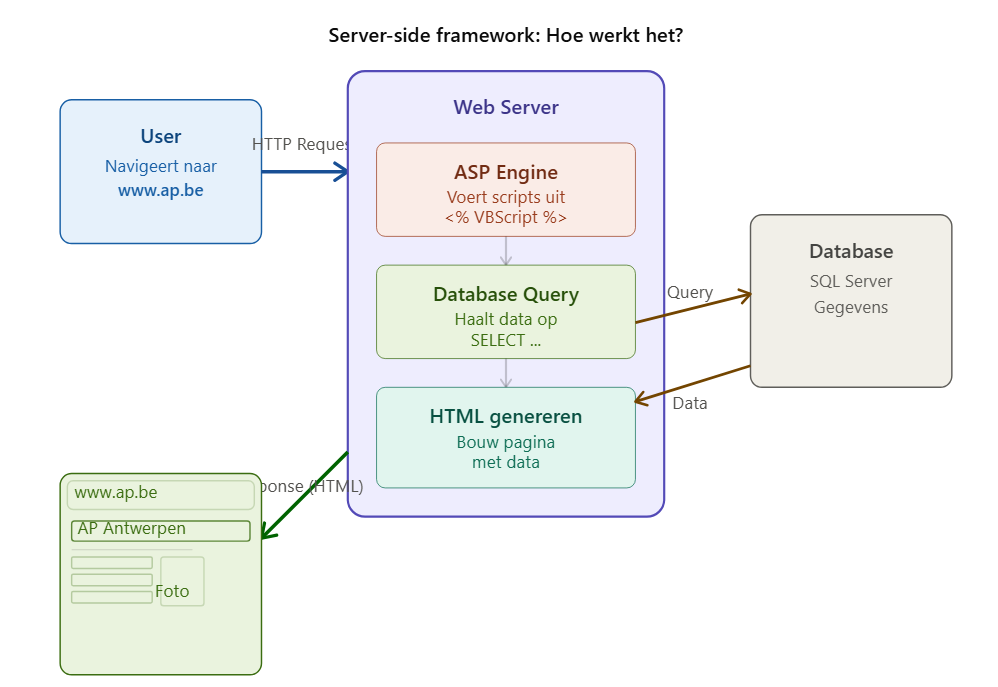
\includegraphics[width=0.8\textwidth]{assets/server_side_framework_with_website.png}
        \captionof{figure}{Server-side framework}
        \label{fig:server-side-framework-pic}
    \end{center}
}

\definition[def:client-side-framework]{Client Side Web Framework}{
    Een client-side framework is een framework waarbij de UI-logica in de browser wordt uitgevoerd met JavaScript. De applicatie wordt in de browser geladen en vraagt daarna zelf gegevens op bij de server, meestal via een Web API die data zoals JSON terugstuurt.
    \begin{center}
        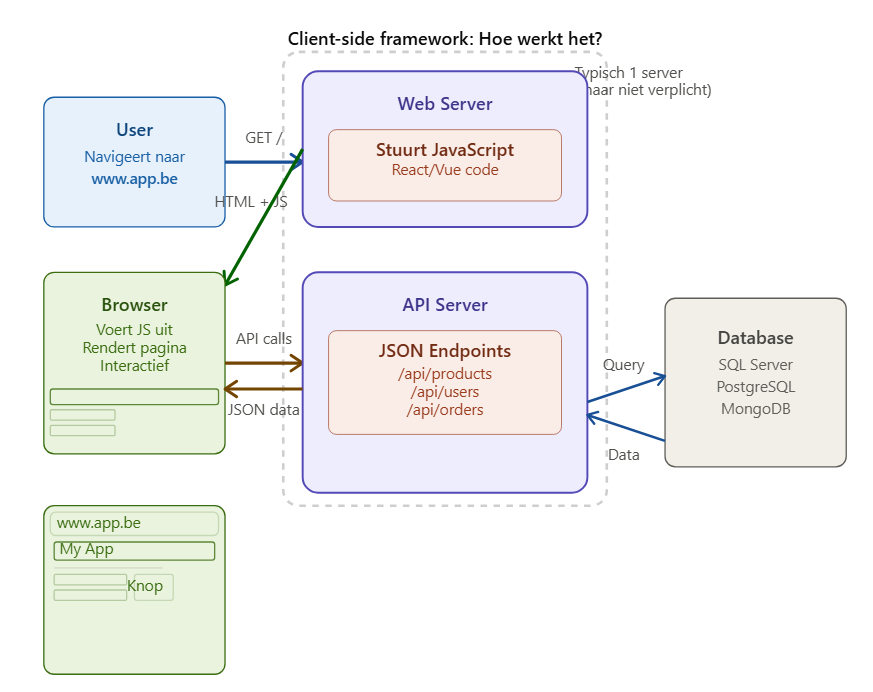
\includegraphics[width=0.8\textwidth]{assets/client_side_framework_with_website.png}
        \captionof{figure}{Client-side framework}
        \label{fig:client-side-framework-pic}
    \end{center}
}

\definition[def:dom]{Document Object Model (DOM)}{
    De DOM is de objectgeoriënteerde representatie van een HTML-pagina in de browser. Elke HTML-tag wordt voorgesteld als een object in een boomstructuur, die door JavaScript kan worden aangepast en door de browser wordt gerenderd.
}

\definition[def:domein]{Domein}{
    Een domein is het deel van een URL dat na \texttt{http://} of \texttt{https://} komt en de website identificeert, bijvoorbeeld \texttt{ap.be}.
}

\definition[def:route]{Route}{
    Een route is het deel van een URL dat na het domein komt en aangeeft welke resource of functionaliteit wordt opgevraagd. Bijvoorbeeld bij \texttt{https://ap.be/api/students} is \texttt{api/students} de route.
}

\definition[def:cors]{CORS}{
    CORS staat voor \textit{Cross-Origin Resource Sharing} en bepaalt of een applicatie resources mag opvragen van een ander domein dan het domein waarop de applicatie zelf gehost wordt.
    \begin{center}
        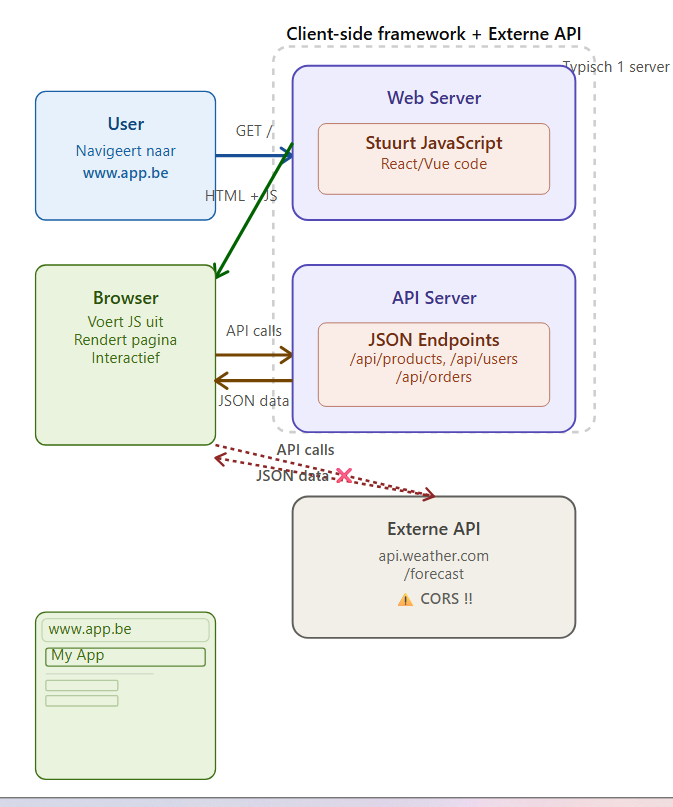
\includegraphics[width=0.8\textwidth]{assets/cors.png}
        \captionof{figure}{Client side framework met externe API en CORS}
        \label{fig:cors-pic}
    \end{center}
}

\section{Evolutie}

\begin{itemize}
    \item \textbf{1996 -- ASP (Active Server Pages):} HTML gecombineerd met server-side scripts om dynamische webpagina's te genereren.
    
    \item \textbf{2002 -- ASP.NET:} server-side code kon geschreven worden in .NET-talen zoals C\# en VB.NET.
    
    \item \textbf{2009 -- ASP.NET MVC:} introduceerde het Model-View-Controller patroon om de applicatie op te splitsen in data (Model), gebruikersinterface (View) en logica (Controller).
    
    \item \textbf{2016 -- ASP.NET Core MVC:} volledig herbouwde, open-source en cross-platform versie van ASP.NET met betere performantie en een modulaire architectuur.
    
    \item \textbf{Vanaf 2017:} ASP.NET Core evolueert samen met de verschillende .NET Core- en later .NET-versies.
\end{itemize}

\definition[def:lts]{LTS}{
    LTS staat voor \textit{Long Term Support}. Een LTS-versie wordt gedurende een langere periode ondersteund met beveiligingsupdates, bugfixes en stabiliteitsverbeteringen, waardoor ze geschikt is voor projecten die langdurig stabiel moeten blijven.
}

\section{API project aanmaken}
\begin{itemize}
    \item \textbf{Program.cs:} het startpunt van de applicatie. Hier wordt de webserver gestart en worden services, dependency injection, middleware en routes geconfigureerd.

    \item \textbf{appsettings.json:} bevat configuratiegegevens van de applicatie, zoals logging en databank-connectiestrings.

    \item \textbf{Controllers/:} bevat de controllers die binnenkomende HTTP-requests verwerken en bepalen welke response wordt teruggestuurd.
\end{itemize}

\section{Controllers}
\subsection{HTTP request, response, middleware en routing}

Een \textbf{HTTP request} bestaat uit drie delen:
\begin{itemize}
    \item \textbf{Request line}: bevat de HTTP-verb en het path.
    \item \textbf{Headers}: extra informatie over de request.
    \item \textbf{Body}: optionele data die naar de server wordt gestuurd.
\end{itemize}

Bijvoorbeeld:

\begin{verbatim}
PUT /api/products/5 HTTP/1.1
Content-Type: application/json

{
    "name": "Umbrella",
    "price": 15.99
}
\end{verbatim}

Een \textbf{HTTP response} bestaat eveneens uit drie delen:
\begin{itemize}
    \item \textbf{Status line}: bevat de HTTP-statuscode.
    \item \textbf{Headers}: extra informatie over de response.
    \item \textbf{Body}: optionele gegevens die worden teruggestuurd.
\end{itemize}

Een binnenkomende request doorloopt eerst de \textbf{middleware pipeline}.
Elke middleware voert een specifieke taak uit en stuurt de request normaal door
naar de volgende middleware. Een middleware kan de request ook stoppen en
zelf onmiddellijk een response terugsturen.

De \textbf{routing middleware} bepaalt uiteindelijk welke controller en action
moeten worden uitgevoerd op basis van de route en HTTP-verb.

\subsection{CRUD-actions, HTTP-verbs en routes}

CRUD staat voor:

\begin{center}
\begin{tabular}{lll}
\textbf{CRUD} & \textbf{HTTP-verb} & \textbf{Attribuut} \\
\hline
Create & POST & \texttt{[HttpPost]} \\
Read & GET & \texttt{[HttpGet]} \\
Update & PUT / PATCH & \texttt{[HttpPut]} / \texttt{[HttpPatch]} \\
Delete & DELETE & \texttt{[HttpDelete]} \\
\end{tabular}
\end{center}

Een controller krijgt typisch een basisroute:

\begin{verbatim}
[Route("api/[controller]")]
[ApiController]
public class BooksController : ControllerBase
{
}
\end{verbatim}

Voor een specifieke resource kan een routeparameter worden toegevoegd:

\begin{verbatim}
[HttpGet("{id}")]
public ActionResult<Book> GetBook(int id)
{
    ...
}
\end{verbatim}

Hierbij wordt de volledige route bijvoorbeeld:

\begin{verbatim}
/api/books/5
\end{verbatim}

Twee actions mogen dezelfde HTTP-verb gebruiken zolang hun routes verschillend zijn.

\subsection{Parameters uit een request halen}

Een client kan extra informatie op verschillende manieren meesturen:

\begin{itemize}
    \item \textbf{Path / Route}: onderdeel van de URL
    \item \textbf{Query string}: parameters achter \texttt{?}
    \item \textbf{Headers}: key/value-informatie
    \item \textbf{Body}: meestal een JSON-object
\end{itemize}

ASP.NET Core voorziet hiervoor attributen:

\begin{itemize}
    \item \texttt{[FromRoute]}: haalt een parameter uit het path.
    \item \texttt{[FromQuery]}: haalt een parameter uit de query string.
    \item \texttt{[FromHeader]}: haalt een waarde uit de headers.
    \item \texttt{[FromBody]}: haalt JSON uit de body en zet deze om naar een object.
\end{itemize}

Voorbeeld:

\begin{verbatim}
[HttpGet]
public ActionResult<IEnumerable<Person>> GetStudents(
    [FromHeader] string? licenseKey,
    [FromQuery] string? name,
    [FromQuery] int? age)
{
    ...
}

[HttpPost]
public ActionResult<Person> CreateStudent(
    [FromBody] Person student)
{
    ...
}
\end{verbatim}

\subsection{ActionResult en HTTP-statuscodes}

Een controller-action kan als returntype \texttt{ActionResult<T>} gebruiken.
Hierdoor kan de action zowel data als een specifieke HTTP-statuscode teruggeven.

Veelgebruikte helper-methodes:

\begin{center}
\begin{tabular}{ll}
\textbf{Helper} & \textbf{Statuscode} \\
\hline
\texttt{Ok(...)} & 200 OK \\
\texttt{Created(...)} & 201 Created \\
\texttt{NoContent()} & 204 No Content \\
\texttt{BadRequest()} & 400 Bad Request \\
\texttt{NotFound()} & 404 Not Found \\
\end{tabular}
\end{center}

Typische CRUD-statuscodes:

\begin{itemize}
    \item GET: \texttt{200 OK}
    \item POST: \texttt{201 Created}
    \item PUT: \texttt{200 OK}
    \item DELETE: \texttt{204 No Content}
\end{itemize}

Voorbeeld:

\begin{verbatim}
[HttpGet("{id}")]
public ActionResult<Book> GetBook(int id)
{
    Book? book = ...;

    if (book == null)
        return NotFound();

    return Ok(book);
}
\end{verbatim}

\subsection{JSON serialisatie}

ASP.NET Core zet C\#-objecten die vanuit een controller worden teruggegeven
automatisch om naar JSON.

Dit noemt men \textbf{serialisatie}.

De omgekeerde bewerking, waarbij JSON wordt omgezet naar een C\#-object,
noemt men \textbf{deserialisatie}.

Bijvoorbeeld:

\begin{verbatim}
return Ok(book);
\end{verbatim}

kan in de HTTP-response automatisch worden:

\begin{verbatim}
{
    "id": 1,
    "title": "The Hobbit"
}
\end{verbatim}

ASP.NET Core zet daarbij automatisch:

\begin{verbatim}
Content-Type: application/json
\end{verbatim}

\subsection{API testen met een .http-bestand}

Een browser kan normaal enkel eenvoudig GET-requests uitvoeren.

Om ook POST-, PUT- en DELETE-requests te testen kan je in Visual Studio
een \texttt{.http}-bestand gebruiken.

Voorbeeld:

\begin{verbatim}
GET https://localhost:7000/api/books

###

GET https://localhost:7000/api/books/5

###

POST https://localhost:7000/api/books
Content-Type: application/json

{
    "title": "The Hobbit",
    "numberOfPages": 310
}

###

DELETE https://localhost:7000/api/books/5
\end{verbatim}

\subsection{Lifecycle van een Controller}

Je maakt een controller-object \textbf{niet zelf aan}.

Wanneer een request overeenkomt met een bepaalde controller en action,
maakt ASP.NET Core automatisch een nieuwe instantie van die controller aan.

Die controller bestaat enkel tijdens de verwerking van die ene request
en response.

Daarna wordt de instantie opnieuw verwijderd.

Hierdoor mag je geen permanente gegevens bewaren in gewone velden
van een controller.